\section{Help-me-carry}
The robot's owner went shopping for groceries and needs help carrying the groceries from the car into the home.

\subsection{Goal}
The robot must help bringing some objects into the arena from outside.

\subsection{Focus}
This test focuses on safe, robust navigation, people following and navigation in unknown environments.

\begin{itemize}[leftmargin=3cm]
  \item[DSPL \& OPL] Test focuses also in Object Detection and Manipulation.
  \item[SSPL] Test focuses also in People Detection and Human-Robot Interaction.
\end{itemize}

\subsection{Setup}
The operator (the robot's owner) has a set of bags (and possibly other objects) that need to be carried from a place outside the arena back inside.

\begin{enumerate}
  \item \textbf{Location:} One of the arenas (apartment) and its surroundings. The apartment is in its normal state. Part of the test is performed outside the arena in a public space.
  \item \textbf{Start:} The robot starts waiting inside the arena.
  \item \textbf{Car:} The car is any landmark chosen (but \emph{not} announced) beforehand outside the arena. Several bags (see \refsec{rule:scenario_objects}) with groceries are located where the car is parked. 
  \item \textbf{Doors:} All doors in the apartment are initially open.
  \item \textbf{Operator:} A \quotes{professional} operator is selected by the TC to act as the operator of the robot. 
  \item \textbf{Uncontrolled environment:} There are no restrictions on other people walking by or standing around throughout the complete task. 
\end{enumerate}

\subsection{Task}
\begin{enumerate}
  \item \textbf{Start:} The robot starts at a designated starting position in the arena, and waits for the \textit{professional} operator. The operator steps in front of the robot and tells it to follow (e.g. by saying \quotes{follow me}). The team is \emph{not} allowed to instruct the operator.

  \item \textbf{Memorizing the operator:} The robot has to memorize the operator. During this phase, the robot may instruct the operator to follow a certain setup procedure.

  \item \textbf{Following the operator:} When the robot signals that it is ready to start, the operator starts walking --in a natural way-- towards the car. Upon arrival, the operator will indicate the robot when they have reached their destination as instructed by the robot (e.g. by saying \quotes{here is the car} or \quotes{stop following me}).

  \newcounter{enumTemp}
  \setcounter{enumTemp}{\theenumi}
  \item {[DSPL \& OPL]} \textbf{Bring the groceries in} \\
  The robot is asked to deliver a bag with groceries  to a specific location (e.g. \quotes{Take this bag to the kitchen table}).
  \begin{enumerate}
    \item \textbf{Bag pick-up:} The robots gets the bag. For this there are several options to achieve this: 
      \textbf{a)} Human puts bag in robot's hand, 
      \textbf{b)} robot picks up bag on floor,
      \textbf{c)} Robot takes bag from operator's hand
    \item \textbf{Bag delivery:} The robot delivers the bag to the instructed destination. It may place the bag on the floor or onto the placement location.\\

    \item \textbf{Asking for help:} Close to the delivery location is another person. The robot must face at them and kindly ask them to help carrying groceries into the house.
  \end{enumerate}

  \setcounter{enumi}{\theenumTemp}
  \item {[SSPL only]} \textbf{Look for help} \\
  The robot is asked to find a person in a given room and ask them to assist carrying the groceries (e.g. \quotes{Look for Louise in the Kitchen and ask her to help us}).
  \begin{enumerate}
    \item \textbf{Entering the house:} While on its way back to the house, the robot deals with different obstacles along it's path.
    \begin{itemize}[leftmargin=3cm]
      \item[\textbf{1st section}] While going back to the house, a person crosses robot's path.
      \item[\textbf{2nd section}] While going back, a person steps in front of the robot and asks it for the time.
    \end{itemize}

    \item \textbf{Find a person:} After reaching the designated room, the robot needs to find a person (there is only one person in the room, the name is meaningless).
  \end{enumerate}

  \item \textbf{Memorizing the \emph{new} operator:} The robot has to memorize the operator that will help. During this phase, the robot may instruct the operator to follow a certain setup procedure.

  \item \textbf{Guiding the operator:} When the robot signals that it is ready to start guiding, the robot guiding the operator to the car. The robot must clearly announce when the destination (the car) is reached.
  \begin{itemize}[leftmargin=3cm]
    \item[DSPL \& OPL] \textbf{Closed door:} Along it's path to the car, the robot will find a closed door (most likely the entrance to the house) that will need to be opened to reach the destination.
    \item[SSPL only] \textbf{Distracted operator:} After leaving the house, the operator is distracted by another person. The robot must re-gain the operator's attention, remind the task, and continue guiding the operator's to the car.
  \end{itemize}

\end{enumerate}

\subsection{Obstacles}
The robot will encounter some obstacles while navigating and the robot must deal and avoid or otherwise deal with the obstacle. 
The possible obstacles are:
\begin{itemize}
  \item \textbf{3D Object:} A hard to see object that requires more than a laser scanner to be detected such as a bar table (wider at its top than on its bottom), rolling chair, lamp, etc.

  \item \textbf{Small object:} Small object. For example, someone has dropped a piece of fruit (like an apple or mandarin) while carrying the groceries inside.

  \item {[DSPL and OPL]} \textbf{Movable Object:} An object blocking the robot's path which the robot can manipulate or push away (such a rolling chair). When interacting with movable objects, the robot must state clearly that the object will be pushed or moved away.

  \item {[SSPL Only]} \textbf{\textit{Smart} obstacle:} A person blocking the robot's path to whom the robot may speak to and kindly ask to move away. When interacting with people, the robot must look at the person and make clear it is speaking with them.
\end{itemize}
%% Possible extensions: 
%% - DONE: allow the operator to tell for each item where it should go
%% - At the destination room, there is a person waving, waiting for the robot to bring the items so (s)he can take them


\subsection{Additional rules and remarks}
\begin{enumerate}
  \begin{minipage}{0.65\textwidth}
  \item \textbf{Asking for passage:} The robot is allowed to (gently) ask individual people to step aside, but it is not allowed to blindly shout at groups of people.

  \item \textbf{Bag handles:} The handles of the bag are always clear and standing up. See Figure \ref{fig:scenario_container_bag} in \refsec{rule:scenario_objects} for bag description. \footnotemark 

  \item \textbf{Bag pick-up:} If the robot can't handover the bag from the operator (i.e.~take it from the operator's hand) it may pick another bag from the surroundings. Additional bags might be either on the floor or on a table. It is expected the robot to actively try to grasp the bag from the operator's hand, and not passively waiting for the bag to be hanged on it. Shall the robot wait for the operator to hang the bag themself, the robot must clearly state it has detected the bag has been placed.

  \item \textbf{Calling the operator back:} During the following phase, when the robot has lost the operator, it may call the operator back once.
  \end{minipage}\hfill%
  \begin{minipage}{0.65\textwidth}
  \end{minipage}\hfill
  \begin{minipage}{0.25\textwidth}
    \vspace{-20pt}
    \begin{figure}[H]
      \centering
      
\includegraphics[width=2cm]{images/help_me_carry_bag.png}%
      \vspace{-10pt}
      \label{fig:storing_groceries}
      %\caption{Example car with groceries.}
      \caption{Paper bag}
    \end{figure}
    \vspace{-10pt}
    \begin{figure}[H]
      \centering
      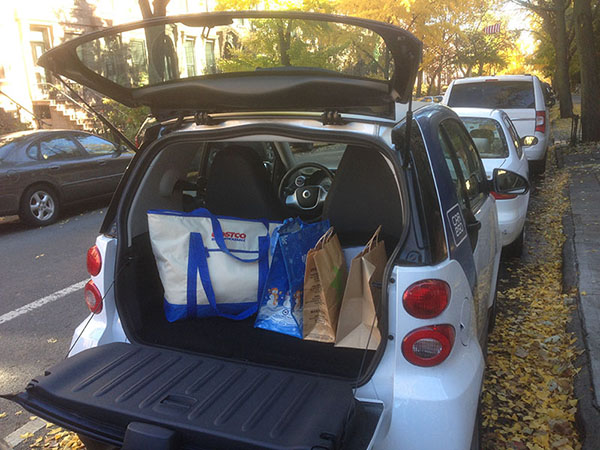
\includegraphics[width=\textwidth]{images/help_me_carry_car.png}%
      \vspace{-20pt}
      \label{fig:storing_groceries}
      %\caption{Example car with groceries.}
      \caption{Car}
    \end{figure}
  \end{minipage}
  \item \textbf{Disturbances from outside:} If a person from the audience (severely) interferes with the robot in a way that makes it impossible to solve the task, the team may repeat the test immediately.

  \item \textbf{Groceries:} Any kind of objects can be found lying around the location designated as the \textit{Car}, such as boxes, sacs, plastic bags, crates, and the groceries itself to give realism to the test. Regardless what objects are present, the robot shall carry an \textbf{official shopping bag} as described below and in \refsec{rule:scenario_objects}.
  
  \item \textbf{Instruction:} The robot interacts with the operator, not the team.
  
  \item \textbf{Natural walking:} The operator has to walk \quotes{naturally}, i.e., move forward facing forward. If not mentioned otherwise, the operator is not allowed to walk back, stand still, signal the robot or follow some re-calibration procedure.

  \item \textbf{Obstacle avoidance:} The robot will encounter several obstacles it must evade on its path between the car and the target destination.
  The robot might be allowed to collide (but not crush) with the small object without the test to be immediately stop. For example, it is allowed to push aside a block of wood, but it won't be allowed to even touch a mandarin or soda can.

  \item \textbf{Opening door:} If unable to open the door, the robot may ask the person being guided to open it (no points are scored).

\end{enumerate}
\footnotetext{This may change in the future. Then, a soft handle may be used which folds down}

\subsection{Data recording}
  Please record the following data (See \refsec{rule:datarecording}):
\begin{itemize}
 \item Maps
 \item Plans
\end{itemize}

\subsection{Referee instructions}

The referee needs to
\begin{itemize}
  \item Distribute some objects over the shopping bags.
  \item Designate a few \quotes{car parking locations} from which the objects must be carried.
\end{itemize}

\subsection{OC instructions}

During setup days
\begin{itemize}
  \item Make bags available.
\end{itemize}

2 hours before the test
\begin{itemize}
  \item Announce the location in which robots will start.
  \item Get and instruct volunteers for the test.
\end{itemize}

\newpage
\subsection{Score sheet}

The maximum time for this test is 4 minutes.

\begin{scorelist}
	\scoreheading{Single iteration}
	\scoreitem[3]{10}{Reach the car}
	\scoreitem[3]{1}{Accept the item from the owner}
	\scoreitem[3]{1}{Understand the commanded destination}
	\scoreitem[3]{6}{Reach inside the arena again}
	\scoreitem[3]{6}{Reach the destination}
	\scoreitem[3]{5}{Put the item at the floor or a nearby table}
	% 3x 30 points = 90 only
	
	% Up to 60 points
	\scoreheading{Obstacle avoidance}
	\scoreitem{5}{Avoiding box-sized object}
	\scoreitem{10}{Avoiding 3D object (Difficult-to-see object)}
	\scoreitem{5}{Asking a person to step aside}
	\scoreitem{30}{Moving away movable object}
	\scoreitem{10}{Move aside for person}
	
	\setTotalScore{150}
\end{scorelist}


% Local Variables:
% TeX-master: "Rulebook"
% End:

